\documentclass[11pt,a4paper]{article}

% ============================================================
% PAQUETES
% ============================================================
\usepackage[utf8]{inputenc}
\usepackage[T1]{fontenc}
\usepackage[spanish]{babel}
\usepackage{geometry}
\geometry{a4paper,margin=2.3cm}
\usepackage{booktabs}
\usepackage{array}
\usepackage{longtable}
\usepackage{graphicx}
\usepackage{caption}
\usepackage{subcaption}
\usepackage{fancyhdr}
\usepackage{listings}
\usepackage{xcolor}
\usepackage{hyperref}
\usepackage{enumitem}
\usepackage{natbib}
\usepackage{amsmath}
\usepackage{tikz}
\usetikzlibrary{arrows.meta,positioning}

\hypersetup{
  colorlinks=true,
  linkcolor=blue!50!black,
  urlcolor=blue!60!black,
  citecolor=blue!50!black,
  pdftitle={Informe tecnico -- Entregable 1 -- ENSO Nino 3.4 / Nino 1+2 -- influencia del cambio climático en los eventos de El Niño y sus impactos en el Perú},
  pdfauthor={Jonathan Paredes}
}

% \url en fuente monoespaciada (igual que \texttt), para nombres de
% archivo/rutas con guiones bajos: \url (a diferencia de \texttt) SI
% permite que LaTeX corte la linea en guiones bajos, puntos y barras,
% evitando "overfull hbox" con rutas largas.
\urlstyle{tt}
% \archivo{...}: como \url{...}, pero en color de texto normal (no el
% urlcolor de los hipervinculos), para que no haya ningun cambio de
% estilo frente al \texttt que reemplaza -- solo cambia el corte de
% linea. Usar con guion bajo LITERAL (no \_) dentro del argumento.
\newcommand{\archivo}[1]{\begingroup\hypersetup{urlcolor=black}\url{#1}\endgroup}

% Columna p{} en modo "ragged right" (sin justificar) para celdas de
% tablas/longtable: el texto justificado en columnas angostas no
% siempre tiene margen para estirarse/encogerse y produce "overfull
% hbox"; en ragged right, LaTeX simplemente corta la linea sin forzar
% el ancho completo.
\newcolumntype{L}[1]{>{\raggedright\arraybackslash}p{#1}}

\definecolor{codebg}{RGB}{247,247,247}
\lstdefinestyle{bashstyle}{
  backgroundcolor=\color{codebg},
  basicstyle=\ttfamily\scriptsize,
  breaklines=true,
  frame=single,
  showstringspaces=false,
  language=bash
}

\pagestyle{fancy}
\fancyhf{}
\fancyhead[L]{\small Entregable 1 -- Influencia del cambio climático en los eventos de El Niño y sus impactos en el Perú}
\fancyhead[R]{\small \thepage}
\renewcommand{\headrulewidth}{0.4pt}

\setlength{\parskip}{0.4em}
\setlength{\parindent}{1.2em}

\begin{document}
\selectlanguage{spanish}

% ============================================================
% PORTADA  (todos los tamaños subidos un nivel)
% ============================================================
\begin{titlepage}
\centering
\vspace*{4cm}

{\LARGE \bfseries Servicio de asistencia en temas de investigación para evaluar la influencia del cambio climático en los eventos de El Niño y sus impactos en el Perú \par}
% \vspace{0.2cm}

\vspace{4cm}

{\LARGE \bfseries Entregable 1 \par}
\vspace{0.5cm}
{\LARGE \bfseries Revisi\'on cient\'ifica, definici\'on conceptual y base de datos \par}
\vspace{0.3cm}

{\large Evaluaci\'on de la se\~nal de cambio clim\'atico en las regiones oceanogr\'aficas Ni\~no~3.4 y Ni\~no~1+2 mediante CMIP6 \par}

\vspace{5cm}

{\Large \textbf{Jonathan Paredes} \par}
{\large Ingeniero Meteor\'ologo \par}
{\normalsize \texttt{japaredesq@gmail.com} \par}

\vspace{0.5cm}

{\normalsize Repositorio: \archivo{https://github.com/Japq91/smn_toe} \par}

\vfill
{\normalsize \today \par}
\end{titlepage}

\tableofcontents
\clearpage
\listoffigures
\listoftables
\clearpage

% ============================================================
\section{Resumen}
% ============================================================

Este informe documenta el Entregable~1 del servicio de asistencia en temas de investigaci\'on de SENAMHI orientado a evaluar la influencia del cambio clim\'atico sobre El Ni\~no-Oscilaci\'on del Sur (ENOS) en las regiones oceanogr\'aficas Ni\~no~3.4 y Ni\~no~1+2. El Entregable~1 cubre exclusivamente la fase de revisi\'on cient\'ifica, definici\'on conceptual y preparaci\'on de la base de datos: no produce a\'un resultados de desempe\~no, proyecci\'on ni \emph{Time of Emergence} (TOE) --esos corresponden a los Entregables~2 a~4--, pero deja construido, verificado y versionado el insumo del que dependen \'integramente.

% REVISAR (redundancia): la cifra "40/102 modelos, 160/160 combinaciones" de
% este párrafo se repite casi palabra por palabra en Datos (Fig. cmip6_contribution),
% en Resultados (inicio de la Sección "Resultados del Entregable 1") y en
% Conclusiones (ítem i). No es incorrecto que el Resumen y las Conclusiones
% adelanten/cierren con la cifra clave, pero las tres repeticiones usan casi
% la misma redacción completa ("40 modelos... 160 combinaciones...").
% Se puede mantener la redacción completa solo en Resultados (donde se
% desglosa el detalle) y, en Resumen/Conclusiones, remitir con una frase corta
% + referencia cruzada en vez de repetir la oración entera.
El resultado operativo de este entregable es un \emph{pipeline} reproducible (repositorio \archivo{smn_toe}, orquestado por un \'unico punto de entrada \texttt{run.sh}) que descarga, homogeneiza, enmascara y valida la variable \texttt{tos} (temperatura superficial del mar, tabla CMOR \texttt{Omon}) de todo modelo CMIP6 disponible con los experimentos \texttt{historical}, \texttt{ssp245} y \texttt{ssp585} -- los exigidos por el TdR para este Entregable (Secci\'on~\ref{sec:alcance}) --, m\'as \texttt{ssp370} como escenario intermedio adicional, junto con la referencia observacional ERSSTv5 de NOAA. Del universo de 102 modelos candidatos (46 de un barrido inicial del vocabulario CMIP6 completo m\'as 56 citados en la literatura del proyecto), 40 modelos quedaron completos en los cuatro experimentos y aprobaron el control de calidad final (160 combinaciones modelo-experimento); el resto qued\'o excluido por descarga incompleta o no disponible en ninguna fuente consultada (Secci\'on~\ref{sec:resultados}). Entre los modelos completos se resolvi\'o, entre otros, un bug de contaminaci\'on num\'erica de FGOALS-f3-L mediante un filtro de seguridad por valor f\'isico (Secci\'on~\ref{sec:paso05}), y cuatro bugs de robustez del propio \emph{pipeline}: paginaci\'on de b\'usqueda de archivos en ESGF que pod\'ia cortarse a mitad ante un corte de red transitorio (Secci\'on~\ref{sec:paso01}), chunks crudos de m\'as de una variante de grilla mezclados en un mismo modelo (Secci\'on~\ref{sec:paso04}), el criterio de selecci\'on del inventario final (Paso~07), que marcaba un modelo como completo si aprobaba el control de calidad de \emph{lo que hab\'ia llegado a intentarse} en vez de exigir expl\'icitamente los cuatro experimentos requeridos -- un modelo con descarga parcial pod\'ia quedar \texttt{selected=True} si esos pocos experimentos igual pasaban QC --, y un cach\'e obsoleto del control de calidad (Paso~06, Secci\'on~\ref{sec:paso06}) que pod\'ia seguir reportando un archivo como \texttt{FAIL} despu\'es de que una redescarga ya lo hubiera corregido.

En paralelo a la construcci\'on del dato, este informe desarrolla el marco te\'orico exigido por los t\'erminos de referencia (TdR): la partici\'on de incertidumbre de \citet{hawkins2012}, su adaptaci\'on por \citet{szabo2016}, el antecedente directo de \citet{bruno2023} sobre CMIP6/Sudam\'erica, el precedente institucional de \citet{alvarez2024}, la caracterizaci\'on del Ni\~no costero de \citet{takahashi2019}, y un estado del arte de otras metodolog\'ias del TOE del cual se deriva la justificaci\'on expl\'icita de los dos m\'etodos de TOE que se aplicar\'an en el Entregable~4: M1 (\citealp{szabo2016}) y \emph{Time of Detection} (ToD, \citealp{gopika2024}).

% ============================================================
\section{Alcance}
\label{sec:alcance}
% ============================================================

Los \textbf{Términos de referencia}: Servicio de asistencia en temas de investigación para evaluar la influencia del cambio climático en los eventos de El Niño y sus impactos en el Perú (en adelante, \textsc{TdR}), define el Entregable~1 --actividad~(a), plazo m\'aximo 25 d\'ias calendario-- como: ``Realizar la revisi\'on de metodolog\'ias sobre tiempo de emergencia (TOE), recopilaci\'on de datos de la informaci\'on de temperatura superficial del mar (TSM), y simulaciones hist\'oricas y futuras de los modelos clim\'aticos globales CMIP6 para los escenarios SSP2-4.5 y SSP5-8.5, correspondientes a las regiones Ni\~no~3.4 y Ni\~no~1+2''. Para operacionalizar este mandato, el equipo t\'ecnico lo descompone en cinco tareas concretas: (i) revisar antecedentes cient\'ificos (ENOS, Ni\~no costero, partici\'on de incertidumbre de Hawkins y Sutton, la aplicaci\'on de Szab\'o, la tesis de Bruno Ram\'irez, el estudio previo de \'Alvarez S\'anchez, y otras metodolog\'ias del TOE); (ii) consolidar el conjunto de modelos CMIP6 disponibles con la variable requerida; (iii) recopilar la referencia observacional ERSSTv5; (iv) definir los dominios oceanogr\'aficos y los periodos temporales de an\'alisis; y (v) homogeneizar unidades, calendarios, resoluciones espaciales y m\'ascaras oc\'eano-tierra entre todas las fuentes. Las tareas (i) son de revisi\'on bibliogr\'afica y se resuelven en la Secci\'on~\ref{sec:marco} de este informe; las tareas (ii)--(v) son computacionales y se resuelven mediante el \emph{pipeline} descrito en las Secciones~\ref{sec:arquitectura} y~\ref{sec:scripts}.
% ============================================================
\section{Revisi\'on cient\'ifica}
\label{sec:marco}
% ============================================================

\subsection{Antecedentes}
\label{sec:antecedentes}

Partici\'on de incertidumbre (Hawkins y Sutton). \citet{hawkins2012} formaliz\'o el \emph{Time of Emergence} como la raz\'on se\~nal-ruido individual por modelo, entendiendo la se\~nal como el ajuste polinomial de la variable de inter\'es y el ruido como la variabilidad interna del residuo. En trabajos relacionados, \citet{hawkins2009,hawkins2011precip} establecieron la partici\'on de la incertidumbre total de una proyecci\'on clim\'atica en tres fuentes independientes: variabilidad interna ($V$, no reducible, propia de la din\'amica ca\'otica del sistema clim\'atico), incertidumbre de modelo ($M$, dispersi\'on entre las respuestas de distintos GCM ante el mismo forzante) e incertidumbre de escenario ($S$, dispersi\'on entre trayectorias de emisiones futuras). Esta partici\'on de tres fuentes es la que el TdR exige aplicar expl\'icitamente en el Entregable~4.

Aplicaci\'on de Szab\'o. \citet{szabo2016} adaptan el m\'etodo de Hawkins y Sutton para temperatura y precipitaci\'on sobre distintas regiones de Europa, introduciendo tres modificaciones que esta propuesta adopta \'integramente como m\'etodo M1 (Secci\'on~\ref{sec:toe_metodos}): la variabilidad interna se recalcula cada a\~no sobre una ventana m\'ovil (no se asume estacionaria), las tres fuentes de incertidumbre se combinan de forma aditiva, y el TOE se define usando \'unicamente la variabilidad interna como ruido de referencia, mientras que la raz\'on se\~nal-ruido s\'i usa la incertidumbre total. Esta es la formulaci\'on que el equipo t\'ecnico adopta (DOI~10.1007/978-3-319-40157-7\_12) para satisfacer el mandato del TdR de calcular la raz\'on se\~nal-ruido y el TOE en el Entregable~4.

% REVISAR (perfumería estilística, no de contenido): este párrafo y el
% siguiente (Álvarez Sánchez) usan la misma fórmula retórica ("es el
% antecedente más directo/institucional de este proyecto"). El contenido de
% ambos párrafos es sustantivo y necesario (justifican metodología y dominio),
% pero la etiqueta evaluativa repetida no aporta información nueva; se podría
% variar la redacción o, si se busca compacidad, quitar la autocalificación
% ("es el antecedente más...") y dejar que el lector lo infiera del contenido.
Tesis de Bruno Ram\'irez. \citet{bruno2023}, trabajo de suficiencia profesional de la Universidad Nacional Agraria La Molina, aplica exactamente la metodolog\'ia de \citet{szabo2016} a temperatura y precipitaci\'on sobre Sudam\'erica usando CMIP6 (54 modelos evaluados), con el mismo periodo de referencia (1981--2010, ajustado a 1981--2014 en este proyecto) y los mismos escenarios (SSP2-4.5/SSP5-8.5) que exige el TdR. Es el antecedente m\'as directo y concreto de este proyecto: la prueba de que el m\'etodo M1 ya fue validado sobre CMIP6 y Sudam\'erica, aunque a escala continental sobre variables terrestres y no a\'un sobre las cajas oceanogr\'aficas Ni\~no~3.4/Ni\~no~1+2 que aqu\'i se abordan. La selecci\'on de modelos de \citet{bruno2023} (validaci\'on f\'isica de sistemas sin\'opticos m\'as validaci\'on estad\'istica contra ERA5: correlaci\'on de Pearson, sesgo, RMSE, diagrama de Taylor) fue el punto de partida conceptual de la consolidaci\'on de modelos de este Entregable~1 (Secci\'on~\ref{sec:datos}), aunque, como se explica en la Secci\'on~\ref{sec:desviacion}, la implementaci\'on final ampli\'o el criterio de selecci\'on a todo el cat\'alogo CMIP6 disponible en vez de partir \'unicamente de esa lista curada.

Estudio previo de \'Alvarez S\'anchez. \citet{alvarez2024}, tambi\'en de la Universidad Nacional Agraria La Molina, proyect\'o cambios de temperatura superficial del mar y nivel del mar en las costas de Sudam\'erica y el Pac\'ifico tropical usando CMIP5. Es el antecedente institucional m\'as directo de este proyecto (mismo dominio oce\'anico, misma casa de estudios) y habilita una comparaci\'on expl\'icita entre generaciones de modelos (CMIP5 vs.\ CMIP6) como parte de la discusi\'on esperada en entregables posteriores.

\textbf{Ni\~no costero.} \citet{takahashi2019} caracterizan din\'amicamente el evento de El Ni\~no costero de 1925, distingui\'endolo de los eventos ``can\'onicos'' de gran escala (1982--1983, 1997--1998): el Ni\~no costero puede desarrollarse con condiciones c\'alidas en el Pac\'ifico oriental lejano y fr\'ias en el Pac\'ifico central, mediado por realimentaciones oc\'eano-atm\'osfera locales (viento-evaporaci\'on-TSM) y no necesariamente por ondas Kelvin ecuatoriales forzadas remotamente.

El TdR pide, en su directiva general para el Entregable~1, la ``revisi\'on de metodolog\'ias sobre tiempo de emergencia (TOE)'', en este sentido se ha revisado tambi\'en metodolog\'ias de TOE m\'as all\'a de Hawkins-Sutton/Szab\'o. 
La Secci\'on~\ref{sec:referencias} sintetiza la \emph{bibliograf\'ia} de referencia --es decir, el conjunto acotado de art\'iculos sobre TOE identificado y revisado para este proyecto, de la cual se deriva adem\'as el m\'etodo complementario ToD (Secci\'on~\ref{sec:toe_metodos}).

\subsection{Literatura sobre \emph{Time of Emergence}}
\label{sec:referencias}

El Cuadro~\ref{tab:referencias} sintetiza la bibliograf\'ia central sobre TOE revisada para este proyecto, incluyendo los antecedentes señalados por el TdR (Secci\'on~\ref{sec:antecedentes}) y literatura de refuerzo incorporada para robustecer la discusi\'on esperada en el Entregable~4.

\begin{longtable}{@{}L{3.6cm}L{3.0cm}L{\dimexpr\textwidth-3.6cm-3.0cm-4\tabcolsep\relax}@{}}
\caption{Bibliograf\'ia sobre \emph{Time of Emergence} usada en este proyecto.}
\label{tab:referencias} \\
\toprule
\textbf{Referencia} & \textbf{Dominio} & \textbf{Aporte principal a este proyecto} \\
\midrule
\endfirsthead
\toprule
\textbf{Referencia} & \textbf{Dominio} & \textbf{Aporte principal a este proyecto} \\
\midrule
\endhead
\citet{hawkins2012} & Global (temperatura del aire en superficie) & Marco se\~nal/ruido fundacional; base del m\'etodo M1 \\
\citet{hawkins2009,hawkins2011precip} & Global (CMIP3) & Origen de la partici\'on en tres fuentes de incertidumbre ($V+M+S$) \\
\citet{szabo2016} & Europa (CMIP3) & M\'etodo M1 adoptado: partici\'on aditiva; TOE con ruido = solo $V$ \\
\citet{bruno2023} & Sudam\'erica, temperatura y precipitaci\'on (CMIP6) & Aplicaci\'on directa del m\'etodo de Szab\'o a CMIP6/Sudam\'erica \\
\citet{alvarez2024} & Costas de Sudam\'erica, Pac\'ifico tropical (CMIP5) & Antecedente institucional directo (UNALM); comparaci\'on CMIP5 vs.\ CMIP6 \\
\citet{takahashi2019} & Pac\'ifico oriental lejano & Caracterizaci\'on din\'amica del Ni\~no costero \\
\citet{gopika2024} & Oc\'eanos tropicales (EEP) & \emph{Time of Detection} (ToD), m\'etodo complementario adoptado \\
\citet{zhong2023} & Pac\'ifico tropical (EEP) & Reg\'imenes de incertidumbre distintos: estado medio vs.\ se\~nal ENOS \\
\citet{larson2025} & Oc\'eano global, fronteras orientales & Circulaci\'on oce\'anica forzada por viento retrasa el TOE de SST \\
\citet{poul2025} & Mar del Norte\slash B\'altico\slash Atl\'antico Norte & F\'ormula S/N \emph{pooled}; \emph{upwelling} retrasa el TOE \\
\citet{keller2014} & Oc\'eano global (biogeoqu\'imica) & TOE observacional; menci\'on expl\'icita de la surgencia Per\'u-Chile \\
\citet{chadwick2019} & Chile central & TOE hidroclim\'atico probabil\'istico; relaci\'on CV--TOE \\
\citet{lois2026} & Oc\'eano Austral & \emph{Storylines} + TOE; principio alternativo de selecci\'on de modelos \\
\citet{giorgi2009} & Precipitaci\'on global (CMIP3) & Origen de la formalizaci\'on S/N; precedente de no emergencia amaz\'onica \\
\bottomrule
\end{longtable}

El hallazgo transversal de esta bibliograf\'ia es que ning\'un m\'etodo de TOE es un est\'andar \'unico: la elecci\'on metodol\'ogica desplaza la fecha resultante en d\'ecadas (comparar, por ejemplo, la partici\'on aditiva de \citealp{szabo2016} frente a la ra\'iz de suma de cuadrados usada en otros trabajos de esa bibliograf\'ia). El equipo t\'ecnico resuelve parcialmente esta ambig\"uedad adoptando el m\'etodo de Szab\'o (Secci\'on~\ref{sec:toe_metodos}), consistente con el mandato general del TdR de calcular la raz\'on se\~nal-ruido y el TOE ``empleando metodolog\'ias revisadas''; este proyecto a\~nade adem\'as el ToD de Gopika como segundo m\'etodo independiente, precisamente para poder reportar un rango de fechas y no un \'unico n\'umero.

\subsection{Similitudes y diferencias entre Ni\~no~3.4 y Ni\~no~1+2}
\label{sec:similitudes}

Siete referencias de la bibliografía merecen una lectura más específica frente al enfoque de este proyecto, más allá de la fila que ocupan en el Cuadro~\ref{tab:referencias}.

\citet{gopika2024} no solo aporta el método ToD adoptado como segunda estimación de TOE: aplica su análisis explícitamente al Pacífico ecuatorial oriental (EEP, por sus siglas en ingles), la caja que geográficamente coincide con Ni\~no~1+2/3.4, y encuentra que es la región de mayor discrepancia modelo-observación de todo el dominio tropical (30°S--30°N): el calentamiento es detectable en el 91\,\% de los modelos CMIP5/6 analizados pero solo en 1 de 4 productos observacionales de SST. Esto sustenta por qué el TdR exige, antes de proyectar, determinar los sesgos de la TSM en el Pacífico tropical central y oriental (Entregable~2): en esta caja específica, la brecha modelo-observación no es un detalle técnico sino el hallazgo central de la literatura de referencia.

\citet{zhong2023} establece una distinción que este proyecto adopta como principio de diseño: usando tres \emph{large ensembles} y CMIP6, muestra que la incertidumbre del TOE del estado medio anual de SST en el EEP está dominada por diferencias entre modelos (la variabilidad interna explica menos del 50\,\%), mientras que la incertidumbre del TOE de la señal ligada al ENOS en la misma caja está dominada por variabilidad interna (77--80\,\% en CESM1-LE). Es decir, el estado medio y la variabilidad de ENOS no comparten el mismo régimen de incertidumbre --exactamente la separación que el TdR exige entre sus objetivos de proyección del estado medio (Entregable~3) y de partición de incertidumbre (Entregable~4).

\citet{larson2025} y \citet{poul2025} documentan, en dos cuencas oceánicas distintas (Pacífico tropical y fronteras orientales; Mar del Norte/Báltico), el mismo mecanismo físico: la circulación oceánica forzada por el viento --particularmente en zonas de surgencia costera-- amplifica el ruido de SST y retrasa sistemáticamente el TOE, en ocasiones impidiendo que la señal emerja del todo dentro del siglo~XXI. \citet{larson2025} menciona explícitamente que, a lo largo de la frontera oriental del Pacífico, la ausencia de señal emergente coincide con regiones de surgencia forzada por viento --la firma física de la Corriente de Humboldt frente a Ni\~no~1+2--. Que dos mecanismos oceánicos independientes converjan en la misma conclusión es la base empírica de la bibliografía para anticipar que Ni\~no~1+2 emergerá más tarde, o de forma más incierta, que Ni\~no~3.4.

\citet{keller2014} reporta la tendencia \emph{observada} de pCO$_2$ en la propia caja Ni\~no~3.4 (1974--2004) como dato de validación independiente, e identifica explícitamente la zona de surgencia de Perú y Chile como una de las regiones oceánicas con TOE localmente elevado ($>$30 años) en variables biogeoquímicas, atribuido a la alta variabilidad natural asociada a ENOS. Es, junto con \citet{larson2025} y \citet{poul2025}, una tercera línea de evidencia independiente --biogeoquímica oceánica en lugar de dinámica física-- que apunta al mismo resultado.

\citet{chadwick2019} es, dentro de la bibliografía, el único precedente de TOE hidroclimático local para Sudamérica (tres cuencas de Chile central) y documenta la relación entre coeficiente de variación (CV) local y fecha de TOE: a mayor CV interanual, TOE más tardío, con retrasos de más de 40 años entre percentiles de tendencia de GCM. 

\citet{lois2026} aporta un principio de selección de modelos distinto al de validación física-estadística de \citet{bruno2023}: en lugar de filtrar por desempeño promedio, selecciona deliberadamente un subconjunto reducido de modelos CMIP6 que acote configuraciones estructurales divergentes. Aplicado a este proyecto, el mismo principio sugiere verificar, en los próximos entregables, que el conjunto final de 40 modelos no colapse artificialmente la dispersión de Índice~C e Índice~E, para no subestimar los porcentajes de las fuentes de incertidumbre y el TOE en Ni\~no~1+2.

% REVISAR (redundancia): este párrafo de cierre re-enumera, con las mismas
% cuatro citas, exactamente lo que cada uno de los cuatro párrafos anteriores
% ya concluyó individualmente (larson2025/poul2025 -> línea 198; keller2014 ->
% línea 200; chadwick2019 -> línea 202; zhong2023 -> línea 196). Es una síntesis
% legítima como cierre de sección, pero tal como está repite casi la misma idea
% cuatro veces en cuatro párrafos y una quinta vez aquí. Se puede acortar a una
% frase de una línea ("estas cuatro líneas convergen en la misma hipótesis:
% Niño~1+2 emergerá más tarde/incierto que Niño~3.4") y dejar que las citas
% completas vivan solo en los párrafos de origen.
En conjunto, cuatro líneas de evidencia independientes de la bibliografía --dinámica oceánica forzada por viento (\citealp{larson2025,poul2025}), biogeoquímica observacional (\citealp{keller2014}), TOE probabilístico hidroclimático (\citealp{chadwick2019}), y separación explícita de regímenes de incertidumbre entre estado medio y ENOS (\citealp{zhong2023})-- convergen en anticipar que \textbf{Ni\~no~1+2 emergerá más tarde o de forma más incierta que Ni\~no~3.4}.

\subsection{Elecci\'on de los dos m\'etodos de \emph{Time of Emergence}}
\label{sec:toe_metodos}

% REVISAR (posible perfumería / desborde de alcance): la Sección~\ref{sec:alcance}
% dice explícitamente que el Entregable~1 NO calcula la partición de
% incertidumbre, la razón señal-ruido ni el TOE (eso es E4). Sin embargo, esta
% subsección desarrolla las cuatro ecuaciones completas de M1 (señal, V(t),
% T(t), umbral de TOE) y la ecuación de ToD con su corrección por autocorrelación
% -- es decir, el aparato matemático completo del método, no solo su
% justificación cualitativa. La propia Sección (línea "el cálculo efectivo de
% ambos métodos corresponde al Entregable~4 y no a este informe") reconoce que
% el cálculo no es de este entregable. Si el objetivo es solo "justificar la
% elección" (lo que pide el TdR en E1), bastaría con explicar en prosa qué mide
% cada método y por qué se eligen ambos (ya está muy bien hecho en el párrafo
% final de esta subsección y en la Cuadro~\ref{tab:metodos_toe}); las ecuaciones
% podrían diferirse al informe del Entregable~4, donde sí se aplican, evitando
% duplicar contenido entre ambos entregables. Si se prefiere mantenerlas aquí
% como adelanto metodológico (razón válida: fija de una vez el método frente al
% cual comparar cuando llegue E4), conviene decirlo explícitamente en una
% frase, en vez de dejar la duplicación implícita.
El TdR exige, para el Entregable~4, calcular la raz\'on se\~nal-ruido y el Tiempo de Emergencia (TOE) ``empleando metodolog\'ias revisadas''; el equipo t\'ecnico adopta para ello, mediante la referencia DOI~10.1007/978-3-319-40157-7\_12, el m\'etodo de \citet{szabo2016}. Este proyecto adopta esa formulaci\'on como m\'etodo M1 y la complementa con un segundo m\'etodo independiente, el \emph{Time of Detection} (ToD) de \citet{gopika2024}, en l\'inea con la revisi\'on de metodolog\'ias de TOE que el TdR pide para el Entregable~1 (Secci\'on~\ref{sec:referencias}). La justificaci\'on de esta elecci\'on doble se desarrolla a continuaci\'on; el c\'alculo efectivo de ambos m\'etodos corresponde al Entregable~4 y no a este informe.

\subsubsection{M\'etodo M1 (Szab\'o y Sz\'epsz\'o)}

Siguiendo a \citet{szabo2016}, quienes adaptan a \citet{hawkins2012} con modificaciones espec\'ificas, la se\~nal se estima ajustando un polinomio de 4\textsuperscript{o} orden a la serie de TSM por modelo $m$ y escenario $s$:
\begin{equation}
\label{eq:szabo_signal}
X_{m,s}(t) = \Delta T_{m,s}(t) + \bar{T} + \varepsilon_{m,s}(t),
\end{equation}
donde $\bar{T}$ es el promedio del ajuste polinomial en el periodo de referencia 1981--2014 (Secci\'on~\ref{sec:dominios_periodos}), $\Delta T_{m,s}(t)$ es la se\~nal de cambio, y $\varepsilon_{m,s}(t)$ es el residuo. La variabilidad interna se calcula, a diferencia de \citet{hawkins2012}, de forma no estacionaria: es la varianza de los residuos recalculada sobre una ventana m\'ovil de 30 a\~nos:
\begin{equation}
\label{eq:szabo_V}
V(t) = \mathrm{var}_{m,s}\big(\varepsilon_{m,s}(\tau)\ \big|\ \tau \in [t-30,\,t]\big).
\end{equation}
La incertidumbre de modelo $M(t)$ y de escenario $S(t)$ se calculan como la varianza entre modelos y entre escenarios de la se\~nal $\Delta T_{m,s}(t)$, respectivamente, y la incertidumbre total es la suma aditiva de las tres fuentes (no la ra\'iz de la suma de cuadrados usada por otros m\'etodos de la bibliograf\'ia):
\begin{equation}
\label{eq:szabo_T}
T(t) = V(t) + M(t) + S(t).
\end{equation}
La raz\'on se\~nal-ruido usa la incertidumbre total, $\mathrm{STN}(t) = G(t)/\sqrt{T(t)}$, mientras que, distintivamente, el TOE usa \'unicamente la variabilidad interna como ruido de referencia:
\begin{equation}
\label{eq:szabo_toe}
\mathrm{TOE} = t \quad \text{tal que} \quad \frac{G(t)}{\sqrt{V(t)}} \geq \kappa, \qquad \kappa \in \{1, 2\},
\end{equation}
con ambos umbrales adoptados por el equipo t\'ecnico para el Entregable~4, siguiendo la misma referencia de \citet{szabo2016}. Esta separaci\'on --STN con ruido total, TOE con ruido puramente interno-- es la caracter\'istica distintiva del m\'etodo de Szab\'o, y no es solo te\'orica para el contexto sudamericano: \citet{bruno2023} ya la implement\'o completa sobre CMIP6 y Sudam\'erica para temperatura y precipitaci\'on, con el mismo periodo de referencia, lo que reduce sustancialmente el riesgo de implementaci\'on de este proyecto.

\subsubsection{M\'etodo M2 complementario ToD (Gopika)}

Como segundo m\'etodo, se adopta el \emph{Time of Detection} de \citet{gopika2024}: en lugar de un umbral se\~nal-ruido fijo, se eval\'ua la significancia estad\'istica del coeficiente de una regresi\'on sobre una ventana temporal creciente $[t_0,T]$, corrigiendo los grados de libertad por la autocorrelaci\'on de la serie:
\begin{equation}
\label{eq:tod}
Y_T(t) = a_T\,W_T(t) + b_T + \varepsilon_T(t), \qquad n_{\text{eff}} = \frac{T-t_0+1}{\sum_\tau r^2(\tau)},
\end{equation}
donde $n_{\text{eff}}$ son los grados de libertad efectivos usados en el test-$t$ de significancia de $a_T$. A diferencia de M1, el ToD no depende de un umbral $\kappa$ arbitrario, sino del nivel de significancia elegido (95\,\% en este proyecto), lo que provee una segunda estimaci\'on de TOE metodol\'ogicamente independiente para contrastar con M1.

% REVISAR (redundancia leve): esta tabla resume en dos columnas exactamente lo
% que las Ecs.~\ref{eq:szabo_toe} y~\ref{eq:tod} y sus párrafos ya explican en
% prosa (ruido de referencia, criterio de TOE de cada método). No sobra como
% tabla-resumen de cierre, pero si se recorta el desarrollo matemático de
% arriba (ver comentario al inicio de la Sección~\ref{sec:toe_metodos}), esta
% tabla podría pasar a ser el resumen principal del método en vez de una
% tercera repetición del mismo contraste M1/ToD.
\begin{table}[htbp]
\caption{Justificaci\'on de los dos m\'etodos de TOE adoptados.}
\label{tab:metodos_toe}
\small
\begin{tabular}{@{}L{2.3cm}L{5.6cm}L{\dimexpr\textwidth-2.3cm-5.6cm-4\tabcolsep\relax}@{}}
\toprule
\textbf{M\'etodo} & \textbf{Ruido de referencia} & \textbf{Criterio de TOE} \\
\midrule
M1 (Szab\'o) & Solo variabilidad interna $V(t)$, ventana m\'ovil de 30 a\~nos & $G(t)/\sqrt{V(t)} \geq \kappa$, $\kappa=1$ o $2$ \\
ToD (Gopika) & Residuo de regresi\'on, grados de libertad efectivos & Significancia del coeficiente sostenida al 95\,\% \\
\bottomrule
\end{tabular}
\end{table}

La elecci\'on de estos dos m\'etodos, y no otros de la bibliograf\'ia (Cuadro~\ref{tab:referencias}), responde a tres criterios: (i) M1 satisface directamente el mandato del TdR de calcular la raz\'on se\~nal-ruido y el TOE para el Entregable~4; (ii) ToD ya fue validado por \citet{gopika2024} exactamente sobre la caja EEP que coincide con Ni\~no~3.4/1+2 (Secci\'on~\ref{sec:similitudes}), a diferencia de otros m\'etodos de esa bibliograf\'ia aplicados a dominios sin relaci\'on directa con ENOS (r\'ios australianos, praderas canadienses, Corea del Sur); y (iii) ambos m\'etodos son conceptualmente independientes entre s\'i --uno basado en raz\'on se\~nal-ruido con partici\'on de incertidumbre, el otro en significancia estad\'istica de una tendencia--, lo que permite reportar en el Entregable~4 un rango de fechas de emergencia en vez de un \'unico n\'umero, mitigando el riesgo, documentado en la Secci\'on~\ref{sec:referencias}, de que ning\'un m\'etodo de TOE sea un est\'andar \'unico.

% ============================================================
\section{Datos}
\label{sec:datos}
% ============================================================

Se usan dos fuentes: (i) CMIP6, salidas de modelo de la variable \texttt{tos} (temperatura superficial del mar, tabla CMOR \texttt{Omon}), obtenidas de la federaci\'on ESGF (\emph{Earth System Grid Federation}) y, de forma complementaria, del servicio Copernicus Climate Data Store (CDS); y (ii) ERSSTv5 (\emph{Extended Reconstructed Sea Surface Temperature}, versi\'on 5) de NOAA, descargada directamente de NOAA PSL, como referencia observacional \'unica de todo el \emph{pipeline}. La Figura~\ref{fig:cmip6_contribution} ilustra la contribuci\'on institucional internacional al conjunto CMIP6 finalmente consolidado.

\begin{figure}[htbp]
\centering
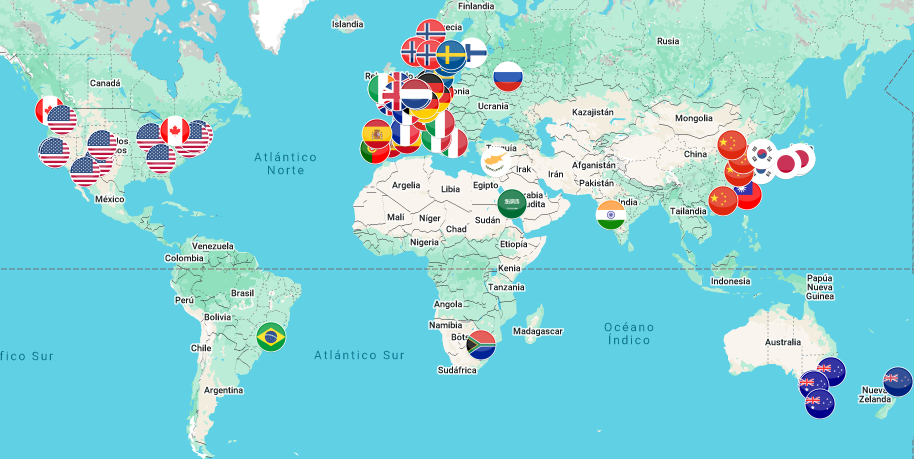
\includegraphics[width=\textwidth]{figuras/cmip6_contribution.png}
\caption[Distribuci\'on institucional de los modelos CMIP6 disponibles por pa\'is de origen.]{Distribuci\'on por instituci\'on/pa\'is de origen de los modelos CMIP6. La dispersi\'on institucional es relevante para la Secci\'on~\ref{sec:similitudes}: un conjunto de modelos concentrado en pocos centros de modelado comparte con mayor probabilidad el mismo sesgo estructural (p.\,ej., lengua fr\'ia o doble ZCIT del Pac\'ifico oriental), lo que subestimar\'ia la incertidumbre real del TOE.}
\label{fig:cmip6_contribution}
\end{figure}

\subsection{Modelos CMIP6 descargados}
\label{sec:tabla_modelos}

El Cuadro~\ref{tab:modelos} lista los 40 modelos CMIP6 seleccionados (Secci\'on~\ref{sec:resultados}: los cuatro experimentos \texttt{historical}, \texttt{ssp245}, \texttt{ssp370} y \texttt{ssp585} completos y aprobados en control de calidad), identificados con el mismo c\'odigo num\'erico \texttt{M001}--\texttt{M102} que usan las Figuras~\ref{fig:qc} y~\ref{fig:mapas2d} y el archivo \archivo{informe/model\_registry.csv} (asignado alfab\'eticamente sobre el universo completo de 102 candidatos, no solo los seleccionados, para que el mismo c\'odigo identifique siempre al mismo modelo en cualquier figura o corrida). Las columnas siguen el orden habitual en tablas de intercomparaci\'on CMIP6: primero la identidad del modelo (c\'odigo, nombre, centro de modelado e instituci\'on/pa\'is de origen que lo public\'o), y despu\'es sus especificaciones t\'ecnicas (realizaci\'on/miembro de ensamble \archivo{variant\_label}, y resoluci\'on nominal). No se repite una columna de experimentos porque, por construcci\'on de la Secci\'on~\ref{sec:resultados}, los 40 modelos de este cuadro tienen exactamente los mismos cuatro completos y aprobados -- la disponibilidad diferenciada por experimento, para el universo completo de 102 candidatos, es la que muestra la Figura~\ref{fig:qc}.

\begin{longtable}{@{}L{1.1cm}L{3.2cm}L{3.2cm}L{2.8cm}L{1.9cm}L{1.9cm}@{}}
\caption[Modelos CMIP6 seleccionados: c\'odigo, centro de modelado, pa\'is, realizaci\'on y resoluci\'on nominal.]{Modelos CMIP6 seleccionados (cuatro experimentos completos y aprobados). C\'odigo \texttt{M001}--\texttt{M102}: identificador num\'erico estable (\archivo{informe/model\_registry.csv}), igual en las Figuras~\ref{fig:qc} y~\ref{fig:mapas2d}. Instituci\'on: identificador \archivo{institution\_id} de CMIP6 del centro de modelado. Pa\'is: derivado del \emph{Controlled Vocabulary} oficial de CMIP6 (\archivo{WCRP-CMIP/CMIP6\_CVs}); para consorcios multinacionales (p.\,ej.\ EC-Earth) es el pa\'is de la sede administrativa, no de todos sus miembros. Realizaci\'on: \archivo{variant\_label} (miembro de ensamble) com\'un a los cuatro experimentos (Secci\'on~\ref{sec:paso01}). Resoluci\'on: \archivo{nominal\_resolution} de la variante de grilla efectivamente descargada -- la m\'as gruesa entre las que publican los cuatro experimentos (Secci\'on~\ref{sec:desviacion}), no la resoluci\'on final compartida tras el regrillado del Paso~04 (\'esa es siempre la de ERSSTv5, $\sim$2\textdegree).}
\label{tab:modelos} \\
\toprule
\textbf{C\'odigo} & \textbf{Modelo} & \textbf{Centro / instituci\'on} & \textbf{Pa\'is} & \textbf{Realizaci\'on} & \textbf{Resoluci\'on} \\
\midrule
\endfirsthead
\toprule
\textbf{C\'odigo} & \textbf{Modelo} & \textbf{Centro / instituci\'on} & \textbf{Pa\'is} & \textbf{Realizaci\'on} & \textbf{Resoluci\'on} \\
\midrule
\endhead
\bottomrule
\endfoot
M001 & ACCESS-CM2 & CSIRO-ARCCSS & Australia & r1i1p1f1 & 250\,km \\
M002 & ACCESS-ESM1-5 & CSIRO & Australia & r1i1p1f1 & 250\,km \\
M007 & AWI-CM-1-1-MR & AWI & Alemania & r1i1p1f1 & 25\,km \\
M010 & BCC-CSM2-MR & BCC & China & r1i1p1f1 & 100\,km \\
M012 & CAMS-CSM1-0 & CAMS & China & r1i1p1f1 & 100\,km \\
M013 & CAS-ESM2-0 & CAS & China & r1i1p1f1 & 100\,km \\
M017 & CESM2 & NCAR & Estados Unidos & r1i1p1f1 & 111\,km \\
M019 & CESM2-WACCM & NCAR & Estados Unidos & r1i1p1f1 & 111\,km \\
M023 & CMCC-CM2-SR5 & CMCC & Italia & r1i1p1f1 & 100\,km \\
M025 & CMCC-ESM2 & CMCC & Italia & r1i1p1f1 & 100\,km \\
M026 & CNRM-CM6-1 & CNRM-CERFACS & Francia & r1i1p1f2 & 100\,km \\
M027 & CNRM-CM6-1-HR & CNRM-CERFACS & Francia & r1i1p1f2 & 25\,km \\
M028 & CNRM-ESM2-1 & CNRM-CERFACS & Francia & r1i1p1f2 & 100\,km \\
M029 & CanESM5 & CCCma & Canad\'a & r1i1p1f1 & 100\,km \\
M030 & CanESM5-1 & CCCma & Canad\'a & r1i1p1f1 & 100\,km \\
M031 & CanESM5-CanOE & CCCma & Canad\'a & r1i1p2f1 & 100\,km \\
M038 & EC-Earth3 & EC-Earth-Consortium & Suecia & r1i1p1f1 & 100\,km \\
M043 & EC-Earth3-Veg & EC-Earth-Consortium & Suecia & r1i1p1f1 & 100\,km \\
M044 & EC-Earth3-Veg-LR & EC-Earth-Consortium & Suecia & r1i1p1f1 & 100\,km \\
M051 & FGOALS-f3-L & CAS & China & r1i1p1f1 & 100\,km \\
M052 & FGOALS-g3 & CAS & China & r1i1p1f1 & 100\,km \\
M056 & GFDL-ESM4 & NOAA-GFDL & Estados Unidos & r1i1p1f1 & 111\,km \\
M057 & GISS-E2-1-G & NASA-GISS & Estados Unidos & r1i1p3f1 & 250\,km \\
M059 & GISS-E2-1-H & NASA-GISS & Estados Unidos & r1i1p3f1 & 250\,km \\
M060 & GISS-E2-2-G & NASA-GISS & Estados Unidos & r1i1p3f1 & 250\,km \\
M069 & IITM-ESM & CCCR-IITM & India & r1i1p1f1 & 250\,km \\
M070 & INM-CM4-8 & INM & Rusia & r1i1p1f1 & 100\,km \\
M071 & INM-CM5-0 & INM & Rusia & r1i1p1f1 & 100\,km \\
M074 & IPSL-CM6A-LR & IPSL & Francia & r1i1p1f1 & 100\,km \\
M077 & KACE-1-0-G & NIMS-KMA & Corea del Sur & r1i1p1f1 & 250\,km \\
M079 & MCM-UA-1-0 & UA & Estados Unidos & r1i1p1f2 & 250\,km \\
M081 & MIROC-ES2L & MIROC & Jap\'on & r1i1p1f2 & 111\,km \\
M082 & MIROC6 & MIROC & Jap\'on & r1i1p1f1 & 100\,km \\
M084 & MPI-ESM1-2-HR & MPI-M & Alemania & r1i1p1f1 & 50\,km \\
M085 & MPI-ESM1-2-LR & MPI-M & Alemania & r1i1p1f1 & 250\,km \\
M087 & MRI-ESM2-0 & MRI & Jap\'on & r1i1p1f1 & 100\,km \\
M094 & NorESM2-LM & NCC & Noruega & r1i1p1f1 & 100\,km \\
M095 & NorESM2-MM & NCC & Noruega & r1i1p1f1 & 100\,km \\
M097 & TaiESM1 & AS-RCEC & Taiw\'an & r1i1p1f1 & 100\,km \\
M100 & UKESM1-0-LL & MOHC & Reino Unido & r1i1p1f2 & 100\,km \\
\end{longtable}

La resoluci\'on nominal es una categor\'ia controlada del vocabulario CMIP6 (no una medida continua), consultada directamente contra el \'indice de b\'usqueda de ESGF para la variante de grilla efectivamente usada por cada modelo (campo \archivo{nominal_resolution} del \emph{dataset}, ya registrado en \archivo{config/models_seed_cmip6.csv} por el Paso~00b). Esta resoluci\'on no es la que finalmente comparten los archivos procesados: el Paso~04 regrilla a todos por igual a la resoluci\'on de ERSSTv5 ($\sim$2\textdegree, Secci\'on~\ref{sec:desviacion}).

\subsection{Selecci\'on inicial de modelos}
\label{sec:desviacion}

El dise\~no original de este entregable tom\'o como punto de partida el conjunto de modelos previamente seleccionados por su desempe\~no en Sudam\'erica en \citet{bruno2023} (54 modelos validados en su trabajo de suficiencia profesional). Esa lista no se conserv\'o como archivo aparte en el repositorio; en su lugar, sus modelos quedaron trazables dentro de los art\'ifactos que s\'i persisten: de los 52 \archivo{source_id} distintos citados en \citet{bruno2023}, 34 coinciden directamente con el barrido autom\'atico completo de CMIP6 (\archivo{config/models_seed_cmip6.csv}), 16 m\'as quedaron registrados como candidatos de fuente alternativa en \archivo{config/models_missing_from_esgf.csv} (Secci\'on~\ref{sec:scripts}, Paso~00c), y 37 de los 52 terminaron formando parte del inventario final de modelos de este Entregable~1. La implementaci\'on de este Entregable~1 parti\'o conceptualmente de esa lista pero la ampli\'o deliberadamente: en lugar de restringir la descarga a esos modelos, el script \archivo{00b_build_model_list.py} (Secci\'on~\ref{sec:scripts}) enumera todos los \archivo{source_id} de CMIP6 publicados en ESGF con \texttt{tos}/\texttt{Omon}, y selecciona los que tienen los cuatro experimentos requeridos. La raz\'on de esta ampliaci\'on es doble: primero, la selecci\'on de \citet{bruno2023} se valid\'o sobre variables terrestres (temperatura del aire, precipitaci\'on) y sistemas sin\'opticos continentales, no sobre TSM oce\'anica en Ni\~no~3.4/1+2, por lo que no hab\'ia garant\'ia de que fuera exhaustiva para este dominio; segundo, ampliar el universo de candidatos a 102 modelos (46 del barrido inicial m\'as 56 citados en la literatura del proyecto, verificados con \archivo{00c_check_paper_models.py}) permite, en el Entregable~2, decidir con datos propios cu\'ales de esos 40 modelos completos son adem\'as representativos del ENOS observado --sin haber descartado de antemano candidatos v\'alidos por seguir estrictamente una lista pensada para otra variable.

De cada modelo se descarga, adem\'as, la variante de grilla (\archivo{grid_label}) m\'as gruesa disponible entre las que publican los cuatro experimentos (script \texttt{00b}), en lugar de la de mayor resoluci\'on: dado que el paso~04 regrilla igualmente todo a la resoluci\'on del dato observado de referencia (ERSSTv5, $\sim$2\textdegree), descargar variantes de alta resoluci\'on no aportar\'ia precisi\'on adicional al resultado final y s\'olo incrementar\'ia innecesariamente el volumen de datos y el tiempo de descarga.

\subsection{Dominios oceanogr\'aficos y Periodos}
\label{sec:dominios_periodos}

Los dominios de an\'alisis, definidos en \texttt{config/domains.yaml} en convenci\'on de longitud 0--360 (usada de forma consistente en todo el \emph{pipeline}, a diferencia de la convenci\'on $-180/180$), son:

\begin{itemize}
\item \textbf{Ni\~no~3.4}: 170\textdegree{}O--120\textdegree{}O, 5\textdegree{}S--5\textdegree{}N (190\textdegree{}--240\textdegree{} en 0--360).
\item \textbf{Ni\~no~1+2}: 90\textdegree{}O--80\textdegree{}O, 10\textdegree{}S--0\textdegree{} (270\textdegree{}--280\textdegree{} en 0--360).
\item Ventana de descarga (envolvente de ambas cajas, con margen para permitir remapeo conservativo sin efectos de borde): 100\textdegree{}E--70\textdegree{}O, 20\textdegree{}S--20\textdegree{}N.
\end{itemize}

\begin{figure}[htbp]
\centering
\includegraphics[width=0.9\textwidth]{figuras/region_nino_proj.png}
\caption[Ubicaci\'on de las cajas oceanogr\'aficas Ni\~no~3.4 y Ni\~no~1+2, y \'area real de datos procesados.]{Regiones oceanogr\'aficas Ni\~no~3.4 (170\textdegree{}O--120\textdegree{}O, 5\textdegree{}S--5\textdegree{}N) y Ni\~no~1+2 (90\textdegree{}O--80\textdegree{}O, 10\textdegree{}S--0\textdegree{}, ambas con doble borde en la figura) sobre el Pac\'ifico tropical oriental, en proyecci\'on Robinson centrada din\'amicamente en el punto medio de Ni\~no~3.4 (\texttt{config/domains.yaml}). El \'area verde es la ventana de descarga real (100\textdegree{}E--70\textdegree{}O, 20\textdegree{}S--20\textdegree{}N, Secci\'on~\ref{sec:dominios_periodos}): todo el dominio efectivamente descargado, regrillado y enmascarado por el \emph{pipeline}. Ni\~no~1+2, adyacente a la costa peruana y a la zona de surgencia de la Corriente de Humboldt, es la caja de mayor relevancia directa para el monitoreo del Ni\~no costero en Per\'u (\citealp{takahashi2019}), mientras que Ni\~no~3.4 es la caja est\'andar internacional del \'Indice Oce\'anico de El Ni\~no (ONI).}
\label{fig:region_nino}
\end{figure}

La Figura~\ref{fig:region_nino} ubica ambas cajas dentro del Pac\'ifico tropical.



Definidos en \texttt{config/periods.yaml}: periodo de referencia/validaci\'on 1981--2014; proyecciones a 2036--2065 (P1) y 2071--2100 (P2); escenarios \texttt{ssp245}, \texttt{ssp370} y \texttt{ssp585} (\texttt{ssp370} se incorpora como escenario intermedio adicional, para robustecer el an\'alisis de sensibilidad entre SSP2-4.5 y SSP5-8.5). El rango temporal completo de descarga es 1850--2100 (\texttt{historical}: 1850--2014; los tres escenarios SSP: 2015--2100). El criterio de selecci\'on de modelos vigente es \'unicamente la disponibilidad de \texttt{tos}/\texttt{Omon} en los cuatro experimentos \texttt{historical}, \texttt{ssp245}, \texttt{ssp370} y \texttt{ssp585}.

% ============================================================
\section{\emph{Pipeline}}
\label{sec:arquitectura}
% ============================================================

Este m\'odulo vive en el repositorio \archivo{smn_toe}, con un \'unico punto de entrada (\texttt{run.sh}) y salidas versionadas en \texttt{data/processed/}, consumibles de forma independiente por el Entregable~2 sin necesidad de conocer el detalle interno de este m\'odulo.

Principios del \emph{pipeline}: idempotencia (cada paso omite su procesamiento si el archivo de salida ya existe, permitiendo interrumpir y reanudar sin recomputar); verificaci\'on por valor y no por metadato (las Secciones~\ref{sec:paso04} y~\ref{sec:paso05} documentan dos casos concretos en que confiar en el atributo declarado de una variable, en vez de en su valor num\'erico real, habr\'ia dejado pasar datos err\'oneos); y cascada de fuentes con degradaci\'on expl\'icita (Secci\'on~\ref{sec:paso02}): un \texttt{git clone} nuevo m\'as \texttt{./run.sh}, sin intervenci\'on manual, obtiene todo lo que sea posible obtener automatizadamente, y deja registrado en el reporte de estado (Secci\'on~\ref{sec:reporte}) qu\'e qued\'o pendiente y por qu\'e.

\subsection{Script principal \texttt{run.sh}}
\label{sec:runsh}

Todo el \emph{pipeline} se ejecuta desde un \'unico punto de entrada, \texttt{run.sh}, ubicado en la ra\'iz del repositorio. Se invoca como \archivo{./run.sh [STEP_FROM] [STEP_TO] [MAX_MODELS]}, con los tres argumentos opcionales: sin argumentos, ejecuta la secuencia completa de pasos (00, 00b, 01, 02, 03, 04, 05, 06 y 07, en ese orden fijo); con los dos primeros argumentos, restringe la ejecuci\'on a un rango de pasos (por ejemplo, \texttt{./run.sh 06 07} repite \'unicamente el control de calidad y el inventario final tras corregir un modelo problem\'atico, sin repetir descargas ni regrillado ya completados); y el tercer argumento, \archivo{MAX_MODELS}, acota opcionalmente el n\'umero de modelos procesados por corrida, \'util para probar el \emph{pipeline} de punta a punta sobre un subconjunto peque\~no antes de lanzarlo sobre el universo completo de modelos.

Internamente, \texttt{run.sh} no contiene l\'ogica de procesamiento propia: para cada paso de la secuencia, invoca al script correspondiente (Secci\'on~\ref{sec:scripts}) solo si el \'indice de ese paso cae dentro del rango \archivo{STEP_FROM}--\archivo{STEP_TO}, y registra su salida est\'andar en \texttt{logs/pipeline.log}. El paso~02 (descarga) se invoca a trav\'es de \archivo{scripts/run_download_if_idle.sh}, que antes de lanzar una nueva descarga verifica si ya hay una en curso en otro proceso del sistema (Secci\'on~\ref{sec:paso02}); esto permite invocar \texttt{run.sh} repetidamente, incluso mientras una descarga anterior sigue en curso, sin riesgo de duplicarla. Al final de cada corrida, sin importar qu\'e rango de pasos se haya ejecutado, \texttt{run.sh} genera adem\'as el reporte de estado descrito en la Secci\'on~\ref{sec:reporte} (\archivo{logs/run_report_<timestamp>.txt}), de modo que cada ejecuci\'on --completa o parcial-- deja constancia verificable de qu\'e modelos quedaron descargados, procesados o pendientes.

\begin{figure}[htbp]
\centering
\begin{tikzpicture}[
  scale=0.95,                    % <-- reduce todo al 75%
  transform shape,               % <-- escala también nodos y texto
  box/.style={draw, rounded corners, fill=green!80!white!10, align=center, text width=4.2cm, minimum height=.8cm, font=\small},
  boxaux/.style={draw, rounded corners, dashed, fill=green!20!cyan!15, align=center, text width=2.6cm, minimum height=1.1cm, font=\small},
  edg/.style={-{Latex[length=3mm]}, thick},
  edgd/.style={-{Latex[length=3mm]}, dashed, gray!80!black},
  every node/.style={font=\small}
]

\node[box] (S00) at (0,0) {00: Entorno};
\node[box] (S00b) at (0,-1.5) {00b: Modelos candidatos};
\node[boxaux] (S00c) at (5.5,-1.5) {00c\\Verif. literatura};
\node[box] (S01) at (0,-3) {01: Cat\'alogo ESGF};

\node[box] (S02) at (-2.6,-4.5) {02: Descarga CMIP6};
\node[box] (S03) at (3.9,-4.5) {03: Descarga ERSSTv5};
\node[box] (S02b) at (-2.6,-6) {02b: Nodos ESGF alt.};
\node[box] (S02c) at (-2.6,-7.5) {02c: Copernicus CDS};

\node[box] (S04) at (0.5,-9) {04: Grilla com\'un};
\node[box] (S05) at (0.5,-10.5) {05: M\'ascara oc\'eano-tierra};
\node[boxaux] (NB) at (5.5,-10.5) {Notebook\\gr\'aficos\\explorat.};
\node[box] (S06) at (0.5,-12) {06: Control de calidad};
\node[box] (S07) at (0.5,-13.5) {07: Inventario final};
\node[box] (S08) at (0.5,-15) {Registro de modelos};
\node[box] (S09) at (0.5,-16.5) {Gr\'aficos autom\'aticos};
% \node[box] (S10) at (0.5,-18) {Reporte + paquete final};

\draw[edg] (S00) -- (S00b);
\draw[edgd] (S00b) -- (S00c);
\draw[edg] (S00b) -- (S01);
\draw[edg] (S01) -- (S02);
\draw[edg] (S02) -- (S02b);
\draw[edg] (S02b) -- (S02c);
\draw[edgd] (S02b) to[bend right=60] (S01);
\draw[edgd] (S02c) to[bend right=80] (S01);
\draw[edg] (S02.west) -- ++(-1.5,0) |- (S04.west);
\draw[edg] (S03) -- (S04);
\draw[edg] (S04) -- (S05);
\draw[edg] (S05) -- (S06);
\draw[edg] (S06) -- (S07);
\draw[edg] (S07) -- (S08);
\draw[edg] (S08) -- (S09);
% \draw[edg] (S09) -- (S10);
\draw[edgd] (S05) -- (NB);

\end{tikzpicture}
\caption[Flujograma del \emph{pipeline} del Entregable~1.]{Flujograma del \emph{pipeline} del Entregable~1. Las flechas s\'olidas son transiciones dentro de la secuencia autom\'atica de \texttt{run.sh} (Secci\'on~\ref{sec:runsh}); las flechas punteadas corresponden a pasos manuales/diagn\'osticos (\texttt{00c}, notebook de gr\'aficos exploratorios) o a la actualizaci\'on que los pasos~02b/02c hacen sobre el cat\'alogo del paso~01 cuando resuelven un modelo por una fuente alternativa. La cascada 02~$\to$~02b~$\to$~02c es autom\'atica dentro del propio paso~02 (\archivo{02_download_all_sources.sh}, Secci\'on~\ref{sec:paso02}): cada fuente se intenta \'unicamente para lo que la anterior no haya resuelto. Tras el paso~07, \texttt{run.sh} ejecuta adem\'as, siempre y sin importar \archivo{STEP_FROM}/\archivo{STEP_TO}: el registro de modelos (\archivo{build_model_registry.py}), los cinco gr\'aficos autom\'aticos (\archivo{scripts/plot_*.py}, Secci\'on~\ref{sec:scripts}) y, por \'ultimo, el reporte de estado (Secci\'on~\ref{sec:reporte}) junto con el paquete \archivo{.tar.gz} de entrega (\archivo{bundle_deliverable_update.py}). El notebook de gr\'aficos exploratorios sigue siendo manual e independiente de esta cadena autom\'atica.}
\label{fig:flujograma}
\end{figure}

% ============================================================
\section{\emph{Pipeline}}
\label{sec:scripts}
% ============================================================

Esta secci\'on describe la l\'ogica de cada script por su nombre y ruta, sin reproducir el c\'odigo completo (disponible en el repositorio \archivo{smn_toe}).
La Figura~\ref{fig:flujograma} esquematiza el flujo de datos entre los pasos descritos en la Secci\'on~\ref{sec:scripts}, equivalente al diagrama de flujo que documenta el mismo \emph{pipeline} en el \texttt{README.md} del repositorio.


\subsection{Paso 00 -- \texttt{scripts/00\_setup\_env.sh}}
Verifica dependencias (\texttt{cdo}, \texttt{wget}, \texttt{python3} con el paquete \texttt{requests}) y crea el esqueleto de carpetas de datos y \emph{logs}. No instala nada: falla temprano con un mensaje claro si falta una herramienta. Correcci\'on de dise\~no: versiones previas de este documento asum\'ian AWS CLI y el bucket \emph{Open Data} de CMIP6 en S3 como v\'ia de descarga; se verific\'o que ese bucket est\'a en formato Zarr (incompatible con CDO) y que no existe un bucket S3 p\'ublico equivalente para ERSSTv5, por lo que la adquisici\'on de datos se hace \'integramente por HTTP directo contra nodos ESGF y NOAA PSL (Pasos~02--03).

\subsection{Paso 00b -- \texttt{scripts/00b\_build\_model\_list.py}}
Enumera, v\'ia facetas de b\'usqueda del nodo principal de ESGF (ORNL -- verificado que conoce exactamente el mismo universo de 102 modelos con \texttt{tos}/\texttt{Omon} que el nodo LLNL usado por el Paso~01), todos los \archivo{source_id} de CMIP6 publicados; para cada uno, exige \texttt{historical} (o su equivalente \texttt{hist-1950} de HighResMIP) publicado, probando nodos ESGF alternativos si el nodo principal no lo tiene indexado, y exige adem\'as los cuatro experimentos SSP configurados bajo una misma \archivo{grid_label} (sin ese respaldo de nodos alternativos), eligiendo la variante de grilla de mayor \archivo{nominal_resolution} (m\'as gruesa, convertida a km reales si el vocabulario la reporta en grados) entre las que cubren los cuatro. Los modelos que califican quedan en \archivo{config/models_seed_cmip6.csv} (Secci\'on~\ref{sec:desviacion}); para \emph{todos} los modelos inspeccionados (no solo los seleccionados) escribe adem\'as \archivo{informe/model_availability_priority.csv}, con disponibilidad 0/1 por experimento y una columna de prioridad de b\'usqueda manual. Idempotente con detecci\'on de cambio: antes de rehacer el barrido completo, compara una consulta barata (cu\'antos modelos con \texttt{tos}/\texttt{Omon} hay ahora) contra la corrida anterior, y solo repite el barrido si cambi\'o.

\subsection{Paso 00c -- \texttt{scripts/00c\_check\_paper\_models.py} (diagn\'ostico, manual)}
Escanea los resúmenes de la literatura del proyecto (\archivo{files_MD/*.md}) en busca de nombres de \archivo{source_id} de CMIP6 citados, y los compara contra \archivo{models_seed_cmip6.csv}. Los modelos citados en alg\'un paper pero ausentes del \emph{seed} se escriben en \archivo{config/models_missing_from_esgf.csv}, candidatos a b\'usqueda por v\'ia alternativa (Pasos~02b--02c). No forma parte de la secuencia autom\'atica de \texttt{run.sh}.

\subsection{Paso 01 -- \texttt{scripts/01\_query\_esgf\_catalog.py}}
\label{sec:paso01}
Para cada modelo del \emph{seed}, consulta el nodo principal de ESGF (LLNL) y determina el \archivo{variant_label} (miembro de ensamble) com\'un a los cuatro experimentos requeridos, prefiriendo \texttt{r1i1p1f1} cuando est\'a disponible. Escribe \archivo{data/interim/models_catalog_status.csv} (estado por modelo: completo o no, fuente, miembro, e \archivo{intentos_busqueda}, un acumulado de reintentos entre corridas, ver Secci\'on~\ref{sec:paso02}) y \archivo{data/interim/esgf_file_urls.json} (URLs de archivo por modelo/experimento). Idempotente todo-o-nada: si el CSV de estado ya existe, el script no vuelve a consultar ESGF en absoluto (ni fusiona ni reconsulta modelos individuales incompletos); para forzar un refresco hay que borrar ese CSV junto con el JSON de URLs.

La b\'usqueda de archivos pagina sobre el \'indice de ESGF (offset/l\'imite) hasta traer la lista completa; se detect\'o en producci\'on que un corte de red transitorio a mitad de esa paginaci\'on se aceptaba en silencio como "la lista completa" de archivos de un modelo, dejando un cat\'alogo marcado \texttt{complete=True} pero con archivos faltantes desde el origen (verificado: la misma b\'usqueda de \texttt{EC-Earth3 historical} encontraba 107, 121 o 165 archivos --165 es el total real-- seg\'un la corrida, sin ning\'un error visible en pantalla). Se corrigi\'o reintentando la paginaci\'on completa desde cero cuando se corta por un error transitorio, tanto aqu\'i como en el Paso~02b.

\subsection{Paso 02 -- descarga en cascada}
\label{sec:paso02}
\archivo{scripts/02_download_all_sources.sh} encadena tres fuentes, cada una como \emph{fallback} autom\'atico de la anterior:
\begin{enumerate}[label=(\alph*)]
\item \archivo{02_download_cmip6_chunks.sh} --
Descarga HTTP directa contra el nodo principal de ESGF, usando las URLs ya resueltas por el Paso~01. Cada mirror se reintenta 3 veces con una pausa corta antes de pasar al siguiente URL candidata (necesario para modelos que publican un archivo por a\~no individual, hasta 165 \emph{requests} solo para \texttt{historical}, donde la probabilidad de al menos un corte transitorio en todo el lote es alta).
\item \archivo{02b_search_alt_esgf_nodes.py} --

Para los modelos que el nodo principal no resolvi\'o, repite la b\'usqueda contra otros \'indices de la federaci\'on ESGF -- CEDA (Reino Unido), DKRZ (Alemania), IPSL (Francia), NSC (Suecia) y NCI (Australia) --, ya que un modelo puede no estar indexado en un nodo espec\'ifico por problemas puntuales de replicaci\'on y s\'i estarlo en otro. Antes de entrar a este paso y al~(c), \texttt{run.sh} pregunta expl\'icitamente si se quiere intentar (l\'imite de 15\,s; sin respuesta, o en una corrida no interactiva, contin\'ua igual, nunca bloquea una corrida desatendida).
\item \archivo{02c_download_copernicus_cds.py} --

\'Ultimo recurso, solo para los modelos de \archivo{config/models_copernicus_available.csv} (la lista de modelos que ofrece el selector del \emph{dataset} \texttt{projections-cmip6} en el sitio de Copernicus; confirma que el modelo existe ah\'i, no que tenga todos los experimentos requeridos --eso lo resuelve intentando la descarga real, y muchos \emph{jobs} fallan con \texttt{RoocsValueError} para modelos de ``cola larga'' que CDS no espeja--). Requiere credenciales personales (\texttt{\textasciitilde/.cdsapirc}); si no est\'an disponibles, el paso se omite sin abortar el resto del \emph{pipeline}.
\end{enumerate}
Ejecutar \texttt{run.sh} pasa por \archivo{scripts/run_download_if_idle.sh}, que verifica mediante \texttt{pgrep} si ya hay una descarga en curso en otro proceso (marcada con \archivo{data/interim/.download_running_flag}) y, de ser as\'i, no lanza una segunda -- \texttt{run.sh} puede invocarse repetidamente sin riesgo de duplicar descargas.

Un modelo que agota (b) y (c) sin resolverse suma 1 a la columna \archivo{intentos_busqueda} del cat\'alogo (Secci\'on~\ref{sec:paso01}); al llegar a 3 intentos en corridas separadas, deja de reintentarse autom\'aticamente hasta que se borre el cat\'alogo a mano.

\subsection{Paso 03 -- \texttt{scripts/03\_download\_ersstv5.sh}}
Descarga ERSSTv5 desde NOAA PSL (HTTPS, NetCDF nativo) una \'unica vez, y recorta con CDO (\texttt{sellonlatbox}, \texttt{selvar}) a la ventana regional de descarga (Secci\'on~\ref{sec:dominios_periodos}).

\subsection{Paso 04 -- \texttt{scripts/04\_process\_to\_common\_grid.sh}}
\label{sec:paso04}
Por modelo y experimento: (0) filtra los chunks crudos de \texttt{data/raw/cmip6/<modelo>/<experimento>/} a \'unicamente los que correspondan a la \archivo{grid_label} registrada en el cat\'alogo (Secci\'on~\ref{sec:paso01}), ignorando cualquier archivo de otra grilla que haya quedado en disco de una descarga anterior -- necesario tras detectar en producci\'on que \texttt{CESM2} ten\'ia chunks de dos grillas (\texttt{gn} y \texttt{gr}) del mismo periodo completo mezclados en la misma carpeta, duplicando cada mes al fusionarlos; (1) descarta con \texttt{selvar,tos} cualquier variable auxiliar del archivo crudo antes de regrillar (necesario porque algunos modelos de malla curvil\'inea, p.\,ej.\ IPSL-CM6A-LR, publican variables auxiliares sin atributo \texttt{coordinates} propio que hacen abortar a CDO); (2) calcula, una sola vez por modelo, pesos de remapeo hacia la grilla de ERSSTv5 con \texttt{gencon} (mallas no estructuradas, p.\,ej.\ AWI-CM-1-1-MR) o \texttt{genbil} (el resto), detectando el tipo de malla con \texttt{cdo griddes}; si el remapeo con los pesos compartidos del modelo falla para un experimento puntual, se recalculan pesos propios de ese experimento como respaldo; (3) fusiona temporalmente (\texttt{mergetime}) los fragmentos ya regrillados de un mismo experimento y recorta al rango temporal correspondiente (\texttt{selyear}); (4) homogeneiza el calendario (asigna \texttt{standard} si falta el atributo); (5) homogeneiza unidades Kelvin~$\to$~grados Celsius verificando el valor num\'erico real y no el atributo declarado: se promedia el campo en la caja Ni\~no~3.4 y solo se resta 273.15 si ese promedio es num\'ericamente compatible con Kelvin ($\geq$100), tras detectar un archivo de GISS-E2-1-G (\texttt{ssp585}) cuyo atributo \texttt{units} declaraba \texttt{degC} pero cuyos valores num\'ericos segu\'ian en Kelvin; (6) verifica que el resultado final tenga exactamente la misma lista de meses (a\~no-mes, no solo el conteo) que prometen los chunks crudos de la grilla correcta ya en disco -- si no coincide (mes perdido o duplicado por el propio proceso de fusi\'on/recorte), descarta el resultado y lo deja para reprocesar en la pr\'oxima corrida. Esta verificaci\'on se hace deliberadamente contra lo que los chunks descargados prometen, no contra un conteo ideal fijo de \texttt{config/periods.yaml}: un modelo puede publicar en ESGF, de forma permanente, menos de lo que este \emph{pipeline} pide (p.\,ej.\ \texttt{CAMS-CSM1-0}: sus tres escenarios SSP terminan en 2099, ESGF nunca va a tener 2100) y esa limitaci\'on real se acepta tal cual, en vez de descartar el modelo en cada corrida sin remedio posible.

\subsection{Paso 05 -- \texttt{scripts/05\_apply\_ocean\_mask.py}}
\label{sec:paso05}
Construye una m\'ascara oc\'eano-tierra derivada directamente de ERSSTv5 (un punto es oc\'eano si tiene al menos un valor v\'alido en alg\'un mes de todo el registro), en vez de usar la variable de fracci\'on de tierra (\texttt{sftlf}) propia de cada modelo -- esto garantiza que todas las fuentes (observaci\'on y todos los modelos del inventario) compartan exactamente la misma huella espacial de puntos v\'alidos/faltantes, condici\'on necesaria para comparaciones punto a punto en entregables posteriores. Reescrito en Python (\texttt{netCDF4}/\texttt{numpy}) tras detectar que la cadena previa en CDO (\texttt{mulc,0} sobre el valor de relleno) propagaba mal la m\'ascara y marcaba como oc\'eano el 100\,\% del dominio, incluida la tierra. Adicionalmente, aplica un filtro de seguridad por valor f\'isico: cualquier punto con $|\text{valor}| > 400$ se vuelve \texttt{NaN} independientemente de la m\'ascara oc\'eano-tierra, tras detectar que FGOALS-f3-L propagaba, en un subconjunto de puntos que ERSSTv5 considera oc\'eano, un valor de relleno mal interpretado por el regrillado ($\sim$10$^{35}$) muy por encima de cualquier TSM f\'isicamente posible; este filtro por valor, y no por metadato, es la salvaguarda final que permiti\'o incorporar ese modelo al inventario aprobado (Secci\'on~\ref{sec:resultados}).

\subsection{Paso 06 -- \texttt{scripts/06\_qc\_checks.py}}
\label{sec:paso06}
Control de calidad autom\'atico por archivo homogeneizado: rango f\'isico de TSM ($-2$ a 39\,\textdegree C) y cobertura temporal esperada por experimento (tolerancia del 10\,\% en \texttt{ssp245}/\texttt{ssp585}; para \texttt{historical} se exige \'unicamente que el registro llegue m\'as all\'a de 1950, ya que algunos modelos v\'alidos --p.\,ej.\ IITM-ESM-- publican \texttt{historical} desde 1900 y no desde 1850). Escribe \archivo{data/processed/qc_report.csv}, recalculando siempre las tres m\'etricas para todos los archivos en cada corrida (sin cach\'e por archivo): una versi\'on anterior s\'i cacheaba resultados por nombre de archivo entre corridas, lo que en producci\'on (HPC) dej\'o un \texttt{FAIL} obsoleto para un modelo que ya hab\'ia sido redescargado y corregido por el Paso~04 -- el \texttt{.nc} en disco ya ten\'ia los meses completos, pero \archivo{qc_report.csv} nunca volv\'ia a evaluarlo. Al ser una operaci\'on barata (reducciones CDO, no descargas ni regrillado, menos de un minuto para el universo de 102 modelos), se elimin\'o el cach\'e en vez de intentar invalidarlo por fecha de modificaci\'on.

\subsection{Paso 07 -- \texttt{scripts/07\_build\_inventory\_report.py}}
Combina el resultado del Paso~06 con metadatos de resoluci\'on de grilla obtenidos directamente con \texttt{cdo griddes}, en el inventario final \archivo{data/processed/models_inventory_final.csv}: un modelo queda \texttt{selected=True} solo si sus cuatro experimentos pasan el control de calidad.

\subsection{Reporte de estado -- \texttt{scripts/generate\_status\_report.py}}
\label{sec:reporte}
Al final de cada corrida de \texttt{run.sh}, sin importar el rango de pasos ejecutado, se genera un reporte de texto plano en \archivo{logs/run_report_<timestamp>.txt} categorizando cada modelo: descargado completo, con descarga parcial, procesado, descargado-pero-sin-procesar, o pendiente v\'ia fuentes alternativas.

% ============================================================
\section{Resultados del Entregable 1}
\label{sec:resultados}
% ============================================================

Del universo de 102 modelos candidatos, 40 completaron los cuatro experimentos requeridos v\'ia descarga y aprobaron el control de calidad final (160 combinaciones modelo-experimento), tras el filtro de seguridad por valor descrito en la Secci\'on~\ref{sec:paso05} y las correcciones de robustez de descarga/verificaci\'on de ESGF descritas en las Secciones~\ref{sec:paso01} y~\ref{sec:paso04}. Del resto, 44 modelos no se encontraron en ninguna fuente consultada (ESGF principal, nodos alternativos ni Copernicus CDS) y quedan descartados estructuralmente; un subconjunto adicional qued\'o con descarga parcial (v\'ia ESGF y/o Copernicus), sin completar los cuatro experimentos (ver la Figura~\ref{fig:qc}).

La Figura~\ref{fig:qc} distingue seis estados posibles por celda (modelo $\times$ experimento): c\'irculo verde relleno (PASS) -- descargado y aprueba el control de calidad del Paso~06; cruz roja (FAIL) -- descargado pero no aprueba el control de calidad; c\'irculo verde hueco (PENDIENTE) -- existe un enlace de descarga vivo pero todav\'ia no se descarg\'o o proces\'o; c\'irculo gris hueco (SIN\_LINK) -- el modelo existe seg\'un el Paso~00b pero el Paso~01 no encontr\'o ning\'un enlace de descarga vivo; c\'irculo naranja hueco (SOLO\_HIST1950, s\'olo en la columna \texttt{historical}) -- el modelo publica \texttt{hist-1950} (HighResMIP, 1950--2014) en vez de \texttt{historical} est\'andar (1850--2014), equivalente para fines de clasificaci\'on pero nunca elegible como \emph{seed} porque esos modelos corren \texttt{highres-future} en vez de los SSP est\'andar y por lo tanto nunca tienen los cuatro experimentos requeridos; y cuadrado rojo (UNAVAILABLE) -- el experimento no existe en absoluto para ese modelo en ning\'un nodo consultado.

\begin{figure}[htbp]
\centering

\includegraphics[width=1\textwidth]{figuras/sst_QD_vf.png}
\caption[Disponibilidad y control de calidad de \texttt{tos}/\texttt{Omon} para los 102 modelos candidatos.]{Matriz de estado, por modelo (c\'odigo \texttt{M001}--\texttt{M102} y nombre, Secci\'on~\ref{sec:tabla_modelos}) y por columna (\texttt{tos}, \texttt{historical}, \texttt{ssp245}, \texttt{ssp370}, \texttt{ssp585}), para el universo completo de 102 modelos candidatos -- leyenda de s\'imbolos en el p\'arrafo anterior. De los 102 candidatos, 40 completan las cinco columnas; el resto queda excluido por al menos una columna sin PASS.}
\label{fig:qc}
\end{figure}

Como verificaci\'on exploratoria de que el dato ya qued\'o correctamente homogeneizado, esta secci\'on compara ERSSTv5 contra los tres modelos de grilla nativa m\'as gruesa entre los 40 seleccionados (ACCESS-CM2, ACCESS-ESM1-5 y GISS-E2-1-G, todos a 250\,km nominal, Cuadro~\ref{tab:modelos}) -- elegidos por ser, \emph{a priori}, los que m\'as suavizado pierden en el regrillado a la grilla de ERSSTv5 (Secci\'on~\ref{sec:paso04}), el caso m\'as exigente para verificar que la homogeneizaci\'on espacial qued\'o bien resuelta. Estas figuras, junto con las de disponibilidad/QC (Figura~\ref{fig:qc}) y las comparativas (Figuras~\ref{fig:boxplot}), las genera autom\'aticamente \texttt{run.sh} al final de cada corrida (\archivo{scripts/plot_*.py}, Secci\'on~\ref{sec:scripts}); \archivo{graficos_exploratorios.ipynb} cubre el mismo contenido de forma interactiva, \'util para explorar variantes puntuales, pero no es necesario correrlo para obtener estas figuras.

\begin{figure}[htbp]
\centering
\begin{subfigure}[t]{0.75\textwidth}

\includegraphics[width=\textwidth]{figuras/sst_2d_ERSSTv5.png}
\end{subfigure}
\hfill
\begin{subfigure}[t]{0.75\textwidth}
\includegraphics[width=\textwidth]{figuras/M001_sst_2d_ACCESS-CM2.png}
\end{subfigure}
\hfill
\begin{subfigure}[t]{0.75\textwidth}
\includegraphics[width=\textwidth]{figuras/M002_sst_2d_ACCESS-ESM1-5.png}
\end{subfigure}
\hfill
\begin{subfigure}[t]{0.75\textwidth}
\includegraphics[width=\textwidth]{figuras/M057_sst_2d_GISS-E2-1-G.png}
\end{subfigure}
\caption[Comparaci\'on espacial de SST: ERSSTv5 vs.\ los tres modelos de grilla m\'as gruesa.]{Comparaci\'on espacial de la temperatura superficial del mar media del periodo hist\'orico com\'un (mes de muestra 1950-12), ya en la grilla, calendario, unidades y m\'ascara oc\'eano-tierra homogeneizados por el \emph{pipeline} (Pasos~04--05). De arriba hacia abajo: observado (ERSSTv5) y los tres modelos de grilla nativa m\'as gruesa entre los seleccionados -- cada panel indica su propia fuente/identificador \texttt{M001}--\texttt{M102} (Cuadro~\ref{tab:modelos}) directamente en el t\'itulo del gr\'afico; esta figura es una verificaci\'on visual de que dicha condici\'on se cumple incluso en el caso m\'as exigente (grilla nativa m\'as gruesa), no un resultado de desempe\~no.}
\label{fig:mapas2d}
\end{figure}

Como segunda verificaci\'on exploratoria, complementaria a la anterior, la Figura~\ref{fig:series} muestra la serie de tiempo completa (\texttt{historical} + los tres escenarios SSP superpuestos) de esos mismos tres modelos en ambas cajas de an\'alisis, y la Figura~\ref{fig:boxplot} compara la dispersi\'on y la mediana hist\'orica de TSM entre ERSSTv5 y los 40 modelos del inventario.

\begin{figure}[htbp]
\centering
\begin{subfigure}[t]{\textwidth}
\includegraphics[width=\textwidth]{figuras/M001_serie_ACCESS-CM2_sst_Nino3.4.png}
\end{subfigure}
\begin{subfigure}[t]{\textwidth}
\includegraphics[width=\textwidth]{figuras/M002_serie_ACCESS-ESM1-5_sst_Nino3.4.png}
\end{subfigure}
\begin{subfigure}[t]{\textwidth}
\includegraphics[width=\textwidth]{figuras/M057_serie_GISS-E2-1-G_sst_Nino3.4.png}
\end{subfigure}
\caption[Series de tiempo de TSM en Ni\~no~3.4 para los tres modelos de grilla m\'as gruesa.]{Serie de tiempo de la TSM promediada en la caja Ni\~no~3.4 (1850--2100), \texttt{historical} (gris) y los tres escenarios SSP superpuestos (Secci\'on~\ref{sec:dominios_periodos}), para los mismos tres modelos de la Figura~\ref{fig:mapas2d} -- cada panel indica su propio modelo/identificador \texttt{M001}--\texttt{M102} (Cuadro~\ref{tab:modelos}) directamente en el t\'itulo del gr\'afico. L\'inea fina con marcador de punto en cada dato mensual real, sin interpolar huecos: un tramo sin puntos es directamente visible como un hueco real de datos (chunk nunca descargado), en vez de quedar disimulado por una l\'inea continua entre dos meses lejanos. Dos l\'ineas horizontales de referencia -- mediana observada de ERSSTv5 (roja, discontinua) y mediana hist\'orica del propio modelo (negra, punteada), ambas sobre el mismo periodo hist\'orico com\'un a ambas fuentes -- permiten leer de un vistazo el sesgo del modelo respecto a lo observado. El eje vertical se fija en 19--35\textdegree C (enteros) en todos los paneles y en ambas cajas, para que la amplitud de la variabilidad sea directamente comparable entre modelos y entre Ni\~no~3.4 y Ni\~no~1+2. La caja Ni\~no~1+2 (no incluida aqu\'i por espacio) se genera de forma an\'aloga en \archivo{figures/<M00X>\_serie\_<modelo>\_sst\_Nino1+2.png}.}
\label{fig:series}
\end{figure}

\begin{figure}[htbp]
\centering
\begin{subfigure}[t]{\textwidth}

\includegraphics[width=\textwidth]{figuras/boxplot_Nino3.4.png}
\caption{Ni\~no~3.4}
\end{subfigure}
\begin{subfigure}[t]{\textwidth}

\includegraphics[width=\textwidth]{figuras/boxplot_Nino1+2.png}
\caption{Ni\~no~1+2}
\end{subfigure}
\caption[Vista previa exploratoria: TSM en Ni\~no~3.4 y Ni\~no~1+2, ERSSTv5 vs.\ modelos.]{Dispersi\'on y mediana de la temperatura superficial del mar en ambas cajas, ERSSTv5 frente a los 40 modelos del inventario, sobre el mismo periodo hist\'orico com\'un. Cada caja se colorea seg\'un el sesgo de su mediana respecto a la mediana observada de ERSSTv5 (mapa divergente rojo--azul, m\'as rojo cuanto m\'as c\'alido que lo observado, m\'as azul cuanto m\'as fr\'io; la l\'inea roja punteada marca la mediana observada como referencia). Se incluye \'unicamente como vista previa exploratoria de que el dato qued\'o correctamente homogeneizado y es ya comparable entre fuentes; la evaluaci\'on formal de desempe\~no hist\'orico (climatolog\'ia, sesgos, diagrama de Taylor, \'indices C/E/ONI/RONI/ICEN) corresponde al Entregable~2.}
\label{fig:boxplot}
\end{figure}
\newpage
% ============================================================
\section{Proximos pasos}
\label{sec:roadmap}
% ============================================================

Para orientar la continuidad del proyecto, el Cuadro~\ref{tab:roadmap} resume, por entregable, las gr\'aficas y comparaciones que el TdR s\'i exige a partir del Entregable~2.

\begin{table}[htbp]
\caption{Gr\'aficas y comparaciones exigidas por el TdR, Entregables~2--4.}
\label{tab:roadmap}
\small
\begin{tabular}{@{}L{2.2cm}L{\dimexpr\textwidth-2.2cm-2\tabcolsep\relax}@{}}
\toprule
\textbf{Entregable} & \textbf{Gr\'aficas / Procesos} \\
\midrule
E2 & Climatolog\'ia y ciclo anual observado vs.\ modelado; mapas de sesgo; m\'etricas estad\'isticas (diagrama de Taylor, \'Indices~C y~E) para seleccionar los modelos con mejor capacidad de representaci\'on del ENOS. \\
E3 & Proyecciones del estado medio y del gradiente zonal del Pac\'ifico bajo SSP2-4.5/SSP5-8.5, para 2036--2065 y 2071--2100; cambios en la variabilidad y en la ocurrencia de eventos extremos del ENOS mediante \'indices como ONI e ICEN. \\
E4 & Estimaci\'on de fuentes de incertidumbre y raz\'on se\~nal-ruido; TOE por los dos m\'etodos adoptados (M1 y ToD) para Ni\~no~3.4 y Ni\~no~1+2; estudio t\'ecnico final con s\'intesis comparativa entre ambas cajas, conclusiones y recomendaciones (incluye la hip\'otesis de asimetr\'ia planteada en la Secci\'on~\ref{sec:similitudes}). \\
\bottomrule
\end{tabular}
\end{table}
El Entregable~1 queda completo y verificable sin depender de ning\'un paso posterior, y el Entregable~2 puede comenzar leyendo \'unicamente \texttt{data/processed/} -- sin necesidad de re-ejecutar ni conocer el detalle interno de este m\'odulo.


\newpage
% ============================================================
\section{Conclusiones}
\label{sec:conclusiones}
% ============================================================

El Entregable~1, en cumplimiento de la actividad~(a) del TdR (Secci\'on~\ref{sec:alcance}), deja construido, verificado y versionado el insumo completo del que depender\'an los Entregables~2 a~4, de su ejecuci\'on se desprenden las siguientes conclusiones:

\begin{enumerate}[label=(\roman*)]

\item El \emph{pipeline} qued\'o completo y verificable: de 102 modelos CMIP6 candidatos, 40 completaron los cuatro experimentos requeridos y aprobaron el control de calidad final (160 combinaciones modelo-experimento), incluyendo la resoluci\'on de un caso real de contaminaci\'on num\'erica (FGOALS-f3-L, Secci\'on~\ref{sec:paso05}) que un control basado \'unicamente en metadatos no habr\'ia detectado.

\item La revisi\'on cient\'ifica exigida por el TdR (Secci\'on~\ref{sec:marco}) profundiza: la bibliograf\'ia revisada (Cuadro~\ref{tab:referencias}) permite justificar, con evidencia expl\'icita lo requerido por el TdR, la adopci\'on de un segundo m\'etodo de TOE (ToD, \citealp{gopika2024}) independiente del prescrito (M1, \citealp{szabo2016}), y arroja una hip\'otesis de trabajo concreta y contrastable para el Entregable~4: cuatro l\'ineas de evidencia independientes de esa bibliograf\'ia convergen en anticipar que Ni\~no~1+2 emerger\'a m\'as tarde, o de forma m\'as incierta, que Ni\~no~3.4 (Secci\'on~\ref{sec:similitudes}).

\item La ampliaci\'on del universo de modelos candidatos m\'as all\'a de la selecci\'on de \citet{bruno2023} (Secci\'on~\ref{sec:desviacion}) deja al Entregable~2 con m\'as informaci\'on, no menos: la decisi\'on de cu\'ales de los 40 modelos completos son adem\'as representativos del ENOS observado en Ni\~no~3.4/1+2 queda pendiente de esa evaluaci\'on de desempe\~no, en lugar de haberse resuelto de antemano por una lista pensada para otras variables.

\item Todo el trabajo qued\'o versionado y es reproducible sin intervenci\'on manual: un \texttt{git clone} del repositorio \archivo{smn_toe} m\'as \texttt{./run.sh} reconstruye el mismo estado documentado en este informe (Secci\'on~\ref{sec:runsh}), y cada corrida deja adem\'as un reporte de estado verificable (Secci\'on~\ref{sec:reporte}).
\end{enumerate}

% ============================================================
\section{Recomendaciones}
\label{sec:recomendaciones}
% ============================================================

Para la continuidad del proyecto hacia los Entregables~2--4, se recomienda:

\begin{itemize}
\item Al iniciar el Entregable~2, evaluar primero la representatividad f\'isica y estad\'istica del ENOS en el conjunto de 40 modelos completos (\'Indices~C y~E, correlaci\'on, sesgo, diagrama de Taylor sobre Ni\~no~3.4/1+2 espec\'ificamente) antes de dar por buena su idoneidad solo por haber pasado el control de calidad de este entregable, que verifica homogeneizaci\'on y no desempe\~no clim\'atico (Secci\'on~\ref{sec:alcance}).
\item Calcular y reportar M1 y ToD siempre en paralelo (Secci\'on~\ref{sec:toe_metodos}), documentando expl\'icitamente en el Entregable~4 los casos en que ambos m\'etodos difieran sustancialmente en la fecha de TOE, en lugar de reportar un \'unico n\'umero -- la bibliograf\'ia revisada (Secci\'on~\ref{sec:referencias}) muestra que esa discrepancia es la norma, no la excepci\'on, entre m\'etodos de TOE.
\end{itemize}

% ============================================================
\newpage
\bibliographystyle{plainnat}
\bibliography{references}

\newpage
\section{Anexos}
\begin{lstlisting}[style=bashstyle,caption={Estructura interna del repositorio \texttt{smn\_toe}.},label={lst:tree}]
smn_toe/
|-- run.sh                                # orquestador (unico punto de entrada)
|-- environment.yml                       # entorno conda (python, cdo, netcdf4, ...)
|-- config/
|   |-- domains.yaml                      # cajas Nino 3.4 / Nino 1+2 / ventana de descarga
|   |-- periods.yaml                      # periodos y escenarios
|   |-- models_seed_cmip6.csv             # lista de modelos generada por 00b
|   |-- models_missing_from_esgf.csv      # candidatos a fuente alternativa (00c)
|   |-- models_no_encontrado_44.csv       # candidatos sin tos/Omon en ninguna fuente
|   |-- models_copernicus_available.csv   # lista blanca de 02c (existencia en CDS)
|   `-- CMIP6_institution_id.json         # CV oficial CMIP6: institution_id -> pais
|-- scripts/
|   |-- 00_setup_env.sh
|   |-- 00b_build_model_list.py           # nodo principal ORNL
|   |-- 00c_check_paper_models.py         # diagnostico, no forma parte de run.sh
|   |-- 01_query_esgf_catalog.py          # nodo principal LLNL
|   |-- 02_download_all_sources.sh        # orquesta 02a/02b/02c en cascada
|   |-- 02_download_cmip6_chunks.sh       # 02a: ESGF, nodo principal
|   |-- 02b_search_alt_esgf_nodes.py      # 02b: ESGF, nodos alternativos
|   |-- 02c_download_copernicus_cds.py    # 02c: Copernicus CDS (lista blanca)
|   |-- run_download_if_idle.sh           # guardia contra descargas duplicadas
|   |-- 03_download_ersstv5.sh
|   |-- 04_process_to_common_grid.sh
|   |-- 05_apply_ocean_mask.py
|   |-- 06_qc_checks.py
|   |-- 07_build_inventory_report.py
|   |-- build_model_registry.py           # informe/model_registry.csv (codigos M001..M102)
|   |-- generate_status_report.py
|   `-- plot_*.py                         # figuras de este informe (Seccion 8)
|-- data/
|   |-- raw/cmip6/, raw/ersstv5/          # datos tal cual se descargan
|   |-- interim/                          # catalogo, pesos, remap
|   `-- processed/masked/, qc_report.csv, models_inventory_final.csv
|-- informe/
|   |-- model_availability_priority.csv   # disponibilidad 0/1 de los 102 candidatos (00b)
|   `-- model_registry.csv                # institucion, pais, resolucion por codigo M
`-- logs/
\end{lstlisting}

\end{document}
